\newpage
\paragraph{Inverse Reinforcement Learning (IRL) [MAX 2]}  \mbox{} \\
Inverse Reinforcement Learning or Inverse Optimal Control is a Learning from Demonstration approach that was introduced in \cite{abbeel2004apprenticeship}. In IRL, starting from a set of expert-demonstrated trajectories, the main goal is to obtain the \textit{Reward function} $R$, which explains the expert behavior. Once $R$ is found, an RL algorithm is run to obtain the policy $\pi^{L}_{\theta}$ (Algorithm \ref{alg:irl}). \begin{algorithm}
\caption{Classic feature matching IRL algorithm}
\label{alg:irl}
\begin{algorithmic}
\label{alg:irl_algorithm}
\Require Dataset of expert trajectories $D = \left \{ \boldsymbol{\tau}^{E}_{i} \right \}^{N}_{i=1}$ 
\Require Reward function $R_{\omega}$, policy $\pi^{L}_{\theta}$ 
\While {policy improves}
    \State Evaluate the state-action visitation frequency $\mu$ of the current policy $\pi^{L}_{\theta}$
    \State Evaluate the objective function $\mathcal{L}$, w.r.t. $\mu$ and the dataset $D$
    \State Update the reward-function parameters $\omega$ based on $\mathcal{L}$
    \State Update the policy $\pi^{L}_{\theta}$ through a RL algorithm, using the updated $r_{\omega}$
\EndWhile
\end{algorithmic}
\end{algorithm}%Algorithm \ref{alg:irl_algorithm} summarizes the classic procedure followed by a IRL method. It is an iterative procedure characterized by two set of parameters, $\omega$ for the reward function, and $\theta$ for the policy $\pi^{L}_{\theta}$. 
An important design choice is related to how parametrize the reward-function, i.e. a \textbf{linear} function of the features \cite{ratliff2006maximum_margin,ziebart2008maximum_entropy} or  a \textbf{non-linear} function of the features \cite{ratliff2009learning_to_search,wulfmeier2015deep_inverse_rl,finn2016guided_cost_learning}.
Generally, the IRL algorithms are characterized by the following problems: \begin{enumerate*}[label=\textbf{(\arabic*)}]
    \item The learning process could be time-consuming and impractical for high-dimensional problems, because of the double-nested optimization procedure.  
    \item The IRL problem is \textit{ill-posed}, since there are different reward-functions that could lead to the same action.
\end{enumerate*}
%\begin{algorithm}
\caption{Classic feature matching IRL algorithm}
\label{alg:irl}
\begin{algorithmic}
\label{alg:irl_algorithm}
\Require Dataset of expert trajectories $D = \left \{ \boldsymbol{\tau}^{E}_{i} \right \}^{N}_{i=1}$ 
\Require Reward function $R_{\omega}$, policy $\pi^{L}_{\theta}$ 
\While {policy improves}
    \State Evaluate the state-action visitation frequency $\mu$ of the current policy $\pi^{L}_{\theta}$
    \State Evaluate the objective function $\mathcal{L}$, w.r.t. $\mu$ and the dataset $D$
    \State Update the reward-function parameters $\omega$ based on $\mathcal{L}$
    \State Update the policy $\pi^{L}_{\theta}$ through a RL algorithm, using the updated $r_{\omega}$
\EndWhile
\end{algorithmic}
\end{algorithm}
\newline To solve the problem of multiple solutions some constraints to the optimization procedure have to be added, based on the constraint type, the two main IRL procedures can be identified: \begin{enumerate*}[label=\textbf{(\alph*)}]
    \item The \textit{Maximum Margin Prediction} (MMP) approach \cite{ratliff2006maximum_margin,ratliff2009learning_to_search}.  
    \item \textit{Maximum Entropy} (Max-Ent) approach \cite{ziebart2008maximum_entropy,wulfmeier2015deep_inverse_rl,finn2016guided_cost_learning}.
\end{enumerate*}
The MMP methods assume that the demonstrated trajectories are optimal and work in a deterministic setting. The aim is to find the cost-function where the reward of the demonstrated trajectories $R(\boldsymbol{\tau}^{E})$ is greater than the reward of all the alternative trajectories $R_{\omega}(\boldsymbol{\tau})$, by a certain margin $m$, i.e. $ \underset{\omega, m}{\max} \ m \  \ s.t. \ R_{\omega}(\boldsymbol{\tau}^{E}) \geq \max (R_{\omega}(\boldsymbol{\tau})) + m$. The main problem with this formulation is that it does not handle the case in which the expert behavior is sub-optimal, leading to an ambiguous notion of margin. To handle this problem the Max-Ent approach has been proposed in \cite{ziebart2008maximum_entropy}. In Max-Ent the goal is to find the reward-function parameters $\psi$ that drives the policy to maximize the entropy, subject to the feature expectation matching, i.e $\underset{\psi}{\max} \ \mathcal{H}(\pi^{r_{\psi}}) \ s.t. \ \ \mathbb{E}_{\pi^{r_{\psi}}}[\mathbf{f}] = \mathbb{E}_{\pi^{*}}[\mathbf{f}]$. The setting based on the Maximum Entropy is the most popular setting in the IRL field since it removes the ambiguous aspects of the previous formulation. In the original work, the reward-function was a linear combination of the features, i.e. $r_{\psi} = \psi^T \mathbf{f}$. This reward formulation is not suited for high-dimensional feature space, which can require the capability to model non-linear reward structures. In \cite{wulfmeier2015deep_inverse_rl}, a deep-network was used to model the reward-function. In this work, the NN maps the feature vector $\textbf{f}$ into the reward value, and trained according to the Maximum-Entropy setting. Experimental results have shown that the NN ability to approximate highly nonlinear reward functions is essentially to successfully solve tasks in high-dimensional discrete state spaces. A generalization to continuous state-space was proposed in \cite{finn2016guided_cost_learning}. In particular, \cite{finn2016guided_cost_learning} faced the problem of learning a cost function in a high-dimensional continuous state space, with \textbf{unknown dynamics}. Indeed, starting from the exponential trajectory distribution $p(\tau) = \frac{1}{Z} \ exp(-c_{\theta}(\tau))$, the main difficulty is the estimation of the partition function $Z$, needed to compute the negative log-likelihood loss function $\mathcal{L}(\theta) = \frac{1}{N} \underset{\tau^{E}_{i} \in D_{demo}}{\sum} c_{\theta}(\tau^{E}_{i}) + \log(Z)$. Since, the dynamic is unknown the idea was to estimate the partition function through the trajectories obtained from the current policy rollouts, with the idea that during the learning of the cost function the current policy drives the distribution towards regions where samples are more useful.%i.e. $\mathcal{L}(\theta) \approx  \frac{1}{N} \underset{\tau^{E}_{i} \in D_{demo}}{\sum} c_{\theta}(\tau^{E}_{i}) +  \log \frac{1}{M} \underset{\tau^{L}_{j} \in D_{samp}}{\sum} \frac{exp(-c_{\theta}(\tau^{L}_{j}))}{q(\tau_{j})}$.
\begin{algorithm}[htbp]
\caption{Guided-Cost-Learning Algorithm \cite{finn2016guided_cost_learning}}
\label{alg:guided_cost_learning}
\begin{algorithmic}
\Require Initial controller $q_{k}(\tau)$ 
\For {i = 1, \dots, N}
    \State Generate $D_{traj}$ from $q_{k}(\tau)$
    \State $\mathcal{D}_{samp} \leftarrow \mathcal{D}_{samp} \bigcup \mathcal{D}_{traj}$
    \State Update the cost-function parameters, using $\mathcal{D}_{samp}$ and $\nabla_{\theta}\mathcal{L(\theta)}$
    \State Update the controller $q_{k+1}(\tau) \leftarrow q_{k}(\tau)$ according to \cite{levine2014lqr_flm} and using $\mathcal{D}_{traj}$
\EndFor
\end{algorithmic}
\end{algorithm}\label{lqr} Starting from these considerations, the Algorithm \ref{alg:guided_cost_learning} was proposed. The controller was obtained as a result of a Linear-Quadratic Regulator (LQR) optimization procedure, which returns a \textit{linear-gaussian policy}, $\pi(a_{t}|s_{t}) = \mathcal{N}(K_{t}s_{t} + k_{t}, S_{t})$, which optimizes a \textit{quadratic-cost function}, $c(s_{t},a_{t}) = \begin{bmatrix} s_{t} \\ a_{t} \end{bmatrix}^{T}C_{t}\begin{bmatrix} s_{t} \\ a_{t} \end{bmatrix} + \begin{bmatrix} s_{t}\\a_{t}\end{bmatrix}^{T} c_{t} + cc_{t}$,under the assumption of \textit{linear-gaussian dynamics} $s_{t+1} \sim P(s_{t+1}|s_{t},a_{t}) = \mathcal{N}(F_{t}\begin{bmatrix}s_{t}\\ a_{t}\end{bmatrix} + f_{t}, \Sigma_{t})$. The cost-function was parameterized according to a Neural Network, and experiments performed on real-robot manipulation tasks such as dish placement and pouring proved the effectiveness of the proposed method, outperforming the classic Max-Ent method.
%\begin{equation}
\label{formula:linear_gaussian_controller}
    \pi(a_{t}|s_{t}) = \mathcal{N}(K_{t}s_{t} + k_{t}, S_{t})
\end{equation}

\begin{equation}
\label{formula:quadratic_cost_function}
c(s_{t},a_{t}) = \begin{bmatrix}
s_{t}
\\ 
a_{t}
\end{bmatrix}^{T}C_{t}\begin{bmatrix}
s_{t}
\\ 
a_{t}
\end{bmatrix} + \begin{bmatrix}
s_{t}
\\ 
a_{t}
\end{bmatrix}^{T} c_{t} + cc_{t}
\end{equation}

\begin{equation}
\label{formula:gaussian_dyn}
s_{t+1} \sim P(s_{t+1}|s_{t},a_{t}) = \mathcal{N}(F_{t}
\begin{bmatrix}
s_{t}
\\ 
a_{t}
\end{bmatrix} + f_{t}, \Sigma_{t})
\end{equation}



\newline Recent method \cite{das2021model_based_irl_from_vd} tried to move IRL towards more complex learning scenario, such as learning a reward function from video-demonstrations. In \cite{das2021model_based_irl_from_vd} the architecture in Figure \ref{fig:model_based_irl} was proposed. The goal was to obtain the parameters of a cost function $C_{\Psi}(\hat{\boldsymbol{\tau}}, z_{goal})$, such that it was possible to derive a sequence of actions by minimizing the cost-function itself, $\textbf{a}_{new} \ = \ \textbf{a} \ - \ \eta \nabla_{a} C_{\Psi}(\hat{\boldsymbol{\tau}}, z_{goal})$, Different cost functions have been proposed, but all with the same objective to reduce the distance between the current predicted keypoints and the goal keypoints configuration. The trajectory $\hat{\boldsymbol{\tau}}$ is a a sequence of predicted states $[\hat{s}_{1}, \dots, \hat{s}_{T}]$, result of a learned dynamic model, $\hat{s}_{t+1} = f_{dyn}(\hat{s}_{t}, a_{t})$. Experimental results have shown that it is possible to learn a cost-function starting from human/robot video demonstrations. However, the proposed setting was tested on a very simple reaching task, proving how a lot of work has to be made in order to prove the effectiveness or ineffectiveness of IRL in complex real-robot manipulation tasks, starting from video demonstrations.
\begin{figure}[htb]
    \centering
    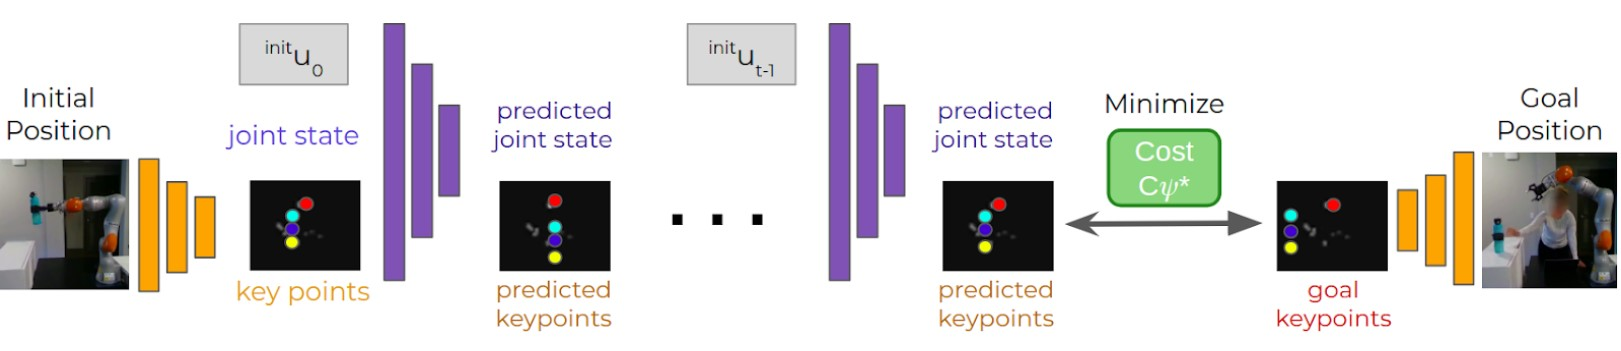
\includegraphics[width=\textwidth]{Figures/images/model_based_irl/model_based_irl.jpg}
    \caption{Architecture proposed in \cite{das2021model_based_irl_from_vd}}
    \label{fig:model_based_irl}
\end{figure}
